%%%
%%% Cours de ``Programmation parallèle''. Polytech'Paris-UPMC
%%% par P. Fortin
%%% revisité par C. Bouillaguet

\documentclass{beamer}
\setbeamerfont{note page}{size=\tiny} % default = small 

\newcommand{\heading}{\frametitle}

\usecolortheme{rose}
\setbeamertemplate{footline}{}
\setbeamertemplate{navigation symbols}{}

\usepackage{amsmath, amssymb, amsthm}
\usepackage{epsfig}
\usepackage[utf8]{inputenc}
\usepackage[french]{babel}
\usepackage[T1]{fontenc}
\usepackage[normalem]{ulem}   
\usepackage{framed}   
\usepackage{tabularx}
\usepackage{url}
\usepackage{psfrag}
\usepackage{alltt}
\usepackage{minted}

\usepackage[formats]{listings}
\lstset{language=C, basicstyle=\scriptsize,showstringspaces=false,extendedchars=true}
\setminted{fontsize=\scriptsize}

%\graphicspath{{Figures/}}

\newtheorem{defi}{Définition}
\newtheorem{lemm}{Lemme}
\newtheorem{exem}{Exemple}
\newtheorem{theor}{Théorème}
\newtheorem{algo}{Algorithme}

\newcommand{\fixme}[1]{{\bf #1}}
\newcommand{\textstruct}[1]{{\color{beamerstructure} #1}}
\newcommand{\textstructbf}[1]{{\color{beamerstructure} \textbf{#1}}}

\newcommand{\mynote}[1]{\note<1>[item]{#1}}

\usepackage{fontspec}

\setsansfont{PalatinoSansLTPro}[
   Path = /home/charles/charles_work/fonts/PalatinoSans/, 
   Extension      = .otf,
   UprightFont    = *-Regular,
   BoldFont= *-Bold ,
   ItalicFont = *-Italic,
   BoldItalicFont = *-BoldIta
]


\author[C.~Bouillaguet]{Charles Bouillaguet \newline
  {\small \texttt{charles.bouillaguet@lip6.fr}}}

\title{Introduction à OpenMP \\ \vspace{1cm} (basé sur diapos de P. Fortin)}
%\date{2020-02-14}

\begin{document}


\begin{frame}
  \titlepage
\end{frame}
  
%%%%%%%%%%%%%%%%%%%%%%%%%%%%%%%%%%%%%%%%%%%%%%%%%%%%%%%%%%%%%%%%%%%%%%%

\begin{frame}
  \frametitle{Threads et processus (rappel)}
  \framesubtitle{Notions de processus et de thread}
  
  Processus : \og flot d'exécution \fg $~+~$ \og espace
  mémoire \fg \\
  Thread : \og flot d'exécution \fg 
  
  \bigskip

  \begin{tabularx}{\textwidth}{X|X}
    Eléments propres & Eléments propres \\
    $\qquad$ à chaque processus & $\qquad$ à chaque thread \\ 
    \hline
    Espace d'adressage & Compteur ordinal \\ 
    Variables globales & Registres \\
    Fichiers ouverts & Pile (dont variables locales)\\
    Processus enfant, signaux\dots & Etat \\
  \end{tabularx}
  
  \bigskip

  \begin{tabularx}{\textwidth}{c|c}
    
\includegraphics[height=0.2\textheight]{multi-processus}$\quad$&
    
\includegraphics[height=0.2\textheight]{multi-thread}\\
    
    Mode multi-processus    &
    $\quad$ Mode multi-thread $\quad$ \\
    
  \end{tabularx}
\end{frame}


%%%%%%%%%%%%%%%%%%%%%%%%%%%%%%%%%%%%%%%%%%%%%%%%%%%%%%%%%%%%%%%%%%%%%%%
\begin{frame}
    \frametitle{Threads et processus (rappel)}

    \begin{columns}[t]
      \column{0.5\textwidth}
      \begin{center}
        Processus mono-thread~:
        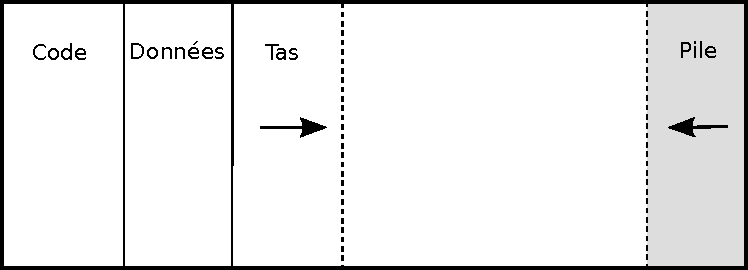
\includegraphics[height=0.2\textheight]{memoire_processus}
      \end{center}
      
      \column{0.5\textwidth}
      \begin{center}
        Processus multi-thread~:
        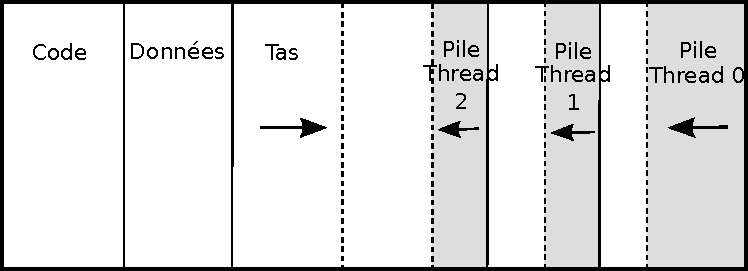
\includegraphics[height=0.2\textheight]{memoire_processus_multi-thread}
      \end{center}
    \end{columns}

\bigskip 

\begin{block}{La mémoire du processus est accessible à tous les threads}
\begin{itemize}

\item Variables \textbf{\alert{partagées}}
  \begin{itemize}
  \item variables \emph{globales} ou \emph{statiques} (segment de données)
  \item variables du tas avec pointeur connu de tous les threads
  \end{itemize}
  
      % $\rightarrow$ Attention aux conflits d'accès à un m\^eme emplacement
      % mémoire ({\it race condition}) ! 
      % Exemple : {\tt i = i + 1 ; }

      
    \item Variables \textbf{\alert{privées}} (à un thread)
      \begin{itemize}
      \item Variables locales (pile),
      \item variables du tas avec pointeur privé
      \end{itemize}
  \end{itemize}
\end{block}
\end{frame}

%%%%%%%%%%%%%%%%%%%%%%%%%%%%%%%%%%%%%%%%%%%%%%%%%%%%%%%%%%%%%%%%%%%%%%%%%


\newcommand{\itemhappy}{\item[{\raisebox{-4pt}{
\includegraphics[height=12pt]{Content}}}]}
\newcommand{\itemsad}{\item[{\raisebox{-4pt}{
\includegraphics[height=12pt]{Triste}}}]}


\begin{frame}
%  \heading{Avantages et inconvénients respectifs d'OpenMP / MPI }

  \begin{block}{OpenMP}
      \begin{itemize}
      \itemhappy plus facile à programmer / mettre au point que MPI
      \itemhappy préserve le code séquentiel original 
      \itemhappy code plus facile à comprendre/maintenir 
      \itemhappy permet une parallélisation progressive 
      \itemsad machines à \alert{mémoire partagée} uniquement
      \itemsad + adapté à certains types de codes (boucles
        parallèles \dots) 
      \end{itemize}
\end{block}

\begin{alertblock}{MPI}
      \begin{itemize}
      \itemhappy s'exécute sur machines à mémoire partagée ou distribuée 
      \itemhappy appliquable plus largement qu'OpenMP
      \itemhappy chaque processus a ses propres variables (pas de conflits)

      \itemsad modifications algorithmiques souvent nécessaires
        %(envoi de messages, recouvrement communications/calcul) 
      \itemsad peut être plus dur à mettre au point 
      \itemsad performance dépend du réseau de communication
      \end{itemize}
\end{alertblock}
  
  
\end{frame}



%%%%%%%%%%%%%%%%%%%%%%%%%%%%%%%%%%%%%%%%%%%%%%%%%%%%%%%%%%%%%%%%%%%%%%%
\begin{frame}
  \frametitle{Historique d'OpenMP}
\begin{itemize}
% \item Échec des différents essais de normalisation

% \item Nécessité de développer un standard pour développer des programmes pour
%   des machines parallèles {\bf à mémoire partagée}

\item 1997, des industriels et des constructeurs adoptent OpenMP ({\it
    Open Multi Processing}) comme un \emph{standard
    industriel}. Interface en Fortran, C et C++


\item Version 2.5 (2000, \texttt{gcc 4.2}) : \emph{lean and mean} (boucles for)

\item Version 3.0 (2008, \texttt{gcc 4.4}) : notion de tâche ({\it task}) 

\item Version 3.1 (2008, \texttt{gcc 4.7}) : rafinements tâche, \texttt{atomic}

\item Version 4.0 (2013, \texttt{gcc 4.9}) : SIMD et \emph{devices} (GPU, ...)

\item Version 4.5 (2013, \texttt{gcc 6}) : raffinement SIMD, GPU, ...

\item Version 5.1 (2020, \texttt{gcc 10}) : \texttt{atomic compare} + ...
  \begin{itemize}
  \item La spec v5.1 est plus dure à lire que la spec v4.5
  \end{itemize}
\end{itemize}

\end{frame}

%%%%%%%%%%%%%%%%%%%%%%%%%%%%%%%%%%%%%%%%%%%%%%%%%%%%%%%%%%%%%%%%%%%%%%%
\begin{frame}
  \frametitle{Principe de base}
\begin{itemize}
  
\item Un processus unique est exécuté sur une machine parallèle à mémoire
  partagée. Le thread correspondant est le thread \og maître \fg~ (de numéro 0).
  
\item Des parties de programme sont exécutés en parallèle par des threads selon
  le modèle {\it fork and join}~:

  \smallskip
  \begin{center}
    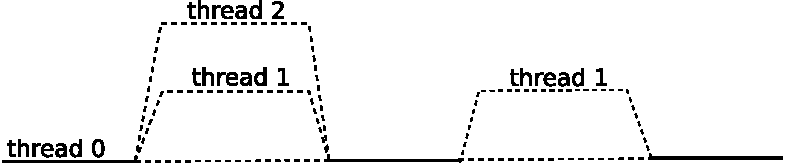
\includegraphics[width=0.9\linewidth]{fork_and_join}
  \end{center}
  \bigskip
  
\item La déclaration des zones parallèles se fait à l'aide de
  directives OpenMP.

\item Modèle mémoire OpenMP particulier : le programmeur peut choisir si une
  variable est {\it privée} ou {\it partagée}.
\end{itemize}

\end{frame}





%%%%%%%%%%%%%%%%%%%%%%%%%%%%%%%%%%%%%%%%%%%%%%%%%%%%%%%%%%%%%%%%%%%%%%%
\begin{frame}
  \frametitle{Utilisation de OpenMP}
  
\begin{itemize}
\item \textbf{Directives de compilation} ({\tt \#pragma} en C)
  \begin{itemize}
  \item Interprétées si le compilateur les reconnaît
  \item Ignorées \alert{silencieusement} sinon
  \item Indiquent au compilateur comment paralléliser le code.
  \item \texttt{gcc} : option \texttt{-fopenmp}
  \end{itemize}

\medskip
  
\item Édition de liens : bibliothèques particulières OpenMP
  \begin{itemize}
  \item \texttt{gcc} : option \texttt{-fopenmp}
  \end{itemize}

\medskip
  
\item Exécution~: des \textbf{variables d'environnement} peuvent être utilisées pour paramétrer
  l'exécution
\end{itemize}
\end{frame}

%%%%%%%%%%%%%%%%%%%%%%%%%%%%%%%%%%%%%%%%%%%%%%%%%%%%%%%%%%%%%%%%%%%%%%

\begin{frame}[fragile]
  \frametitle{OpenMP résumé en une diapo}

  \begin{framed}
    \begin{minted}{C}
// prologue séquentiel
#pragma omp parallel for
for (int i = 0 ; i < n ; i++) {
  /*
   * ici une boucle où toutes les itérations
   * peuvent être exécutées en parallèle.
   */
}
// épilogue séquentiel
\end{minted}
\end{framed}

\texttt{gcc \alert{-fopenmp} prog\_omp.c -o prog\_omp}

\medskip

\begin{itemize}
\item Programme séquentiel \og normal\fg{} jusqu'à \texttt{\#pragma omp}
\item Une \textbf{équipe de threads} est créée
\item Les itérations de la boucle sont \textbf{réparties} entre eux
\item \textbf{Barrière} à la fin de la boucle for
\item Programme séquentiel \og normal\fg{} ensuite
%\item Sans \texttt{\alert{-fopenmp}} : programme purement séquentiel équivalent
\end{itemize}

\end{frame}


% %%%%%%%%%%%%%%%%%%%%%%%%%%%%%%%%%%%%%%%%%%%%%%%%%%%%%%%%%%%%%%%%%%%%%%%
% \begin{frame}[fragile]
%   \frametitle{Création d'un programme OpenMP}


%   \begin{columns}[t]
%     \column{0.5\textwidth}

%     \underline{{\tt test.c}~:}
% \begin{minted}{C}
% int main()
% {
%   #pragma omp parallel 
%   {
%     printf("En parallele !\n");    
%     printf("Toujours //  !\n");    
%   }

%   printf("En sequentiel.\n");
% }
% \end{minted}

% \column{0.5\textwidth}

% \underline{{\tt test2.c}~:}
% \begin{minted}{C}
% int main()
% {
%   #pragma omp parallel 
%   printf("En parallele !\n");    

%   printf("En sequentiel.\n");
% }
% \end{minted}
% \end{columns}
% \end{frame}


% %%%%%%%%%%%%%%%%%%%%%%%%%%%%%%%%%%%%%%%%%%%%%%%%%%%%%%%%%%%%%%%%%%%%%%%
% \begin{frame}[fragile]
%   \frametitle{Compilation et exécution}

% Compilation 

% \begin{center}
% \begin{verbatim}
% \end{verbatim}
% \end{center}

% Exécution 1~:

% \begin{center}
% \begin{verbatim}
% $ ./test2
% En parallele ! 
% En sequentiel.
% \end{verbatim}
% \end{center}

% Exécution 2~:

% \begin{center}
% \begin{verbatim}
% $ export OMP_NUM_THREADS=4
% $ ./test2_openmp
% En parallele ! 
% En parallele ! 
% En parallele ! 
% En parallele ! 
% En sequentiel.
% \end{verbatim}
% \end{center}

% \mynote{{\bf Si OMP\_NUM\_THREADS non définie alors détection automatique
%   du nombre de processeurs/c{\oe}urs (avec OpenMP de gcc).}}

% \end{frame}



%%%%%%%%%%%%%%%%%%%%%%%%%%%%%%%%%%%%%%%%%%%%%%%%%%%%%%%%%%%%%%%%%%%%%%%
\begin{frame}[fragile]
  \frametitle{Compilation conditionnelle et fonctions OpenMP}

\mynote{Peut etre que quelques rappels sur le préprocesseur en C sont nécessaires\dots}

\begin{block}{Compilation conditionnelle}
\begin{minted}{C}
#ifdef _OPENMP
    // Code inclus uniquement si le compilateur supporte OpenMP
    // Dans gcc, seulement si -fopenmp a été utilisé
#endif
\end{minted}
\end{block}


\begin{block}{Fonctions OpenMP}
  Avec \verb|#include <omp.h>|

\begin{itemize}
\item Permettent un mode de programmation SPMD
\item \verb|omp_get_num_threads()|
\item \verb|omp_get_thread_num()|
\item \verb|omp_set_num_threads()|
\item ...
\end{itemize}
\end{block}

\end{frame}



%%%%%%%%%%%%%%%%%%%%%%%%%%%%%%%%%%%%%%%%%%%%%%%%%%%%%%%%%%%%%%%%%%%%%%%
\begin{frame}[fragile]
  \frametitle{Hello world}

\small

\begin{columns}[t]
  \column{6cm}
  
\begin{block}{Programme}
\begin{minted}{C}
#ifdef _OPENMP
#include <omp.h>
#endif

int main()
{
  #pragma omp parallel 
  {
    #ifdef _OPENMP
    printf("Hello world thread %d/%d\n",
          omp_get_thread_num(),
          omp_get_num_threads());
    #else 
    printf("Hello world\n");    
    #endif
  }
}
\end{minted}
\end{block}

\column{4cm}

\begin{block}{Exécution}
\scriptsize
\begin{verbatim} 
$ gcc hello.c -o hello
$ ./hello
Hello world
$ gcc -fopenmp hello.c \
 -o hello
$ export OMP_NUM_THREADS=4
$ ./hello
Hello world thread 0/4
Hello world thread 3/4
Hello world thread 1/4
Hello world thread 2/4
\end{verbatim}
\end{block}  
\end{columns}
\normalsize  

\mynote{Ordre d'exécution quelconque des threads OpenMP.}

\end{frame}




%%%%%%%%%%%%%%%%%%%%%%%%%%%%%%%%%%%%%%%%%%%%%%%%%%%%%%%%%%%%%%%%%%%%%%%
\begin{frame}
  \frametitle{Les directives OpenMP}

Elles sont délimitées par une sentinelle~:

\begin{framed}
  {\tt \#pragma omp} {\it directive [clause[[, ]clause]...]}   
\end{framed}
 
Par défaut, il y a une \textbf{barrière} de synchronisation à la fin. 

\medskip

\begin{block}{Utilisation des directives OpenMP:}
\begin{itemize}
\item débranchement externe interdit ! (\sout{goto}, \sout{setjmp/longjmp}, ...)
\item une seule directive par {\tt \#pragma omp}
\item majuscule/minuscule importante

\item les directives sont : {\tt parallel, for, sections, section, single, master, critical,
  barrier, atomic, flush, ordered, threadprivate, ...}
\end{itemize}
\end{block}

\end{frame}




%%%%%%%%%%%%%%%%%%%%%%%%%%%%%%%%%%%%%%%%%%%%%%%%%%%%%%%%%%%%%%%%%%%%%%%
\begin{frame}
  \frametitle{Le modèle mémoire OpenMP}

  \begin{block}{Rappel}
    \textbf{Variable} : \alert{identifiant} qui désigne une \alert{adresse en mémoire}
  \end{block}
  
  \begin{columns}[t]
    \column{0.5\textwidth}

    Les variables du code source séquentiel original peuvent \^etre
    partagées ({\it shared}) ou privées ({\it private}) en OpenMP. 

    \medskip
    
    \begin{itemize}
    \item {\bf Variable partagée} : chaque thread accède à la variable originale (même adresse). 

    \item {\bf Variable privée} : chaque thread a sa propre \alert{copie} %%locale
      de la variable originale (à des adresses différentes)
    \end{itemize}
    
    \column{0.5\textwidth}
    \begin{center}
      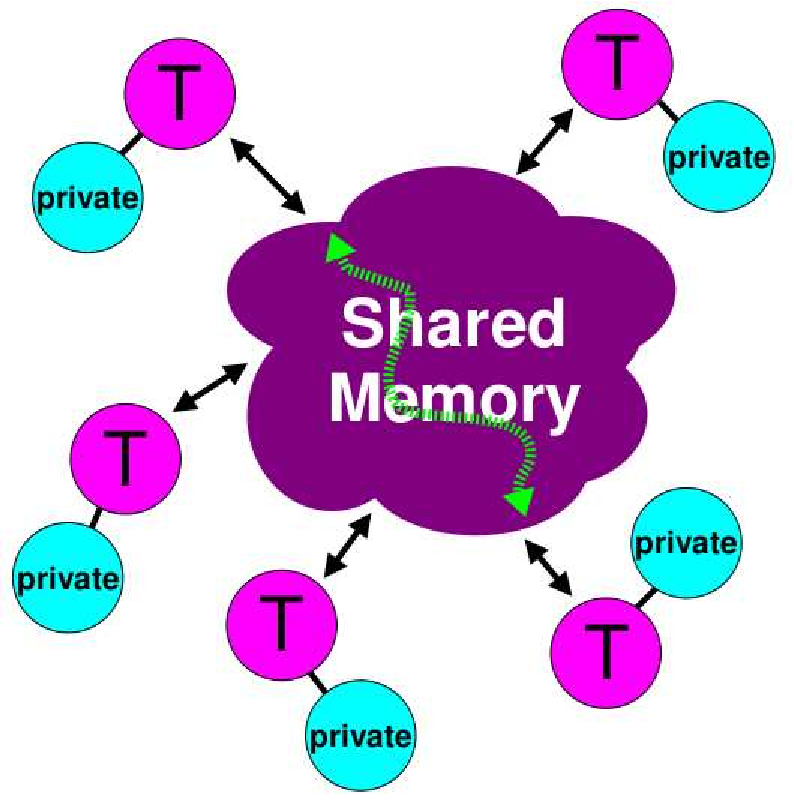
\includegraphics[width=\textwidth]{modele_mem_OpenMP}    

      {\tiny (d'après {\it An Overview of OpenMP 3.0}, R. van der Pas)} 
    \end{center}
  \end{columns}


\end{frame}



%%%%%%%%%%%%%%%%%%%%%%%%%%%%%%%%%%%%%%%%%%%%%%%%%%%%%%%%%%%%%%%%%%%%%%%
\begin{frame}
  \frametitle{Le modèle mémoire OpenMP (suite)}

  \begin{itemize}

  \item Les variables déclarées \textbf{avant} la région parallèle sont
    \textbf{partagées par défaut}

      \medskip
      
    \item On peut modifier leur statut avec  des \alert{clauses} dans les directives OpenMP
      \begin{itemize}
      \item {\tt private, shared, firstprivate, lastprivate, default(shared),
          default(none), reduction, copyin}
      \end{itemize}

      \medskip
      
    \item Les variables locales à un thread sont privées (cf. infra)
      
    \end{itemize}  
\end{frame}



%%%%%%%%%%%%%%%%%%%%%%%%%%%%%%%%%%%%%%%%%%%%%%%%%%%%%%%%%%%%%%%%%%%%%%%
\begin{frame}
  \frametitle{Directive {\tt parallel}}

\begin{framed}
  {\tt \#pragma omp parallel } {\it  [clause[[, ]clause]...]} \\
  {\it bloc structuré} 
\end{framed}

\begin{itemize}
\item Assemble une \alert{équipe de threads} (création/recyclage)   
\item Ils exécutent \textbf{tous} le  {\it bloc structuré}.
\end{itemize}

\begin{block}{Liste des clauses associées à cette directive~:}

\begin{itemize}
\item {\tt if(cond)}: {\tt cond == False} $\rightarrow$ pas de threads
  \begin{itemize}
  \item Par ex. ne pas lancer toute la machine si problème trop petit
  \end{itemize}
  
\item  {\tt private} ({\it var\_list}), {\tt firstprivate} ({\it
    var\_list})

\mynote{{\tt copyin} uniquement pour les variables déclarées comme
  {\tt threadprivate} (voir plus loin)}

\item {\tt reduction} (cf. infra)
  
\item  {\tt num\_threads}({\it int}) : force le nombre de
  threads de l'équipe 

\end{itemize} 
\end{block}
\end{frame}
 


%%%%%%%%%%%%%%%%%%%%%%%%%%%%%%%%%%%%%%%%%%%%%%%%%%%%%%%%%%%%%%%%%%%%%%%
\begin{frame}[fragile]
  \frametitle{}

\begin{minted}{C}
int main()
{
    ...
    initialisation();
    #pragma omp parallel ...
    {
         calcul();
    }
    post_calcul();
}
\end{minted}

\begin{exampleblock}{Possibilités pour définir le nombre de threads}
Par ordre de priorité décroissante~:

\small
\begin{tabular}[ht]{|l@{~:~}l|}
\hline
\#pragma &   \#pragma omp parallel num\_threads(16) \\
\hline
au cours de l'execution &  {\it omp\_set\_num\_threads(4)} \\
\hline
variable d'environnement &  export OMP\_NUM\_THREADS=4 \\
\hline
\end{tabular}
\normalsize
\end{exampleblock}
\end{frame}



%%%%%%%%%%%%%%%%%%%%%%%%%%%%%%%%%%%%%%%%%%%%%%%%%%%%%%%%%%%%%%%%%%%%%%%
\begin{frame}[fragile]
  \frametitle{Les variables prédéfinies sont partagées par défaut}
  
  \begin{columns}[t]
  \column{5cm}
\begin{block}{Programme}
\begin{minted}{C}
#include <omp.h>
#include <stdio.h>

int main()
{
  int c=0;

  #pragma omp parallel 
  {
    c++;
    printf("c=%d thread %d\n",
        c, omp_get_thread_num());
  }
}
\end{minted}
\end{block}
    
    
    \column{5cm}
\begin{block}{Exécution}    
  \small

\begin{verbatim}
$ export OMP_NUM_THREADS=4
$ ./a.out
c=1 thread 3
c=2 thread 0
c=3 thread 1
c=4 thread 2
\end{verbatim}
\end{block}    
  \end{columns}
\end{frame}



%%%%%%%%%%%%%%%%%%%%%%%%%%%%%%%%%%%%%%%%%%%%%%%%%%%%%%%%%%%%%%%%%%%%%%%
\begin{frame}[fragile]
  \frametitle{Attention aux conflits ! }
  
  \small
  \begin{columns}[t]
  \column{5cm}
\begin{block}{Programme}
\begin{minted}{C}
#include <omp.h>
#include <stdio.h>

int main()
{
  int c = 0;

  #pragma omp parallel
  {  
    for (int i=0; i<100000; i++)
        c++;
    printf("c=%d thread %d\n", 
        c, omp_get_thread_num());
  }
}
\end{minted}
\end{block}
    
    
    \column{5cm}
\begin{block}{Exécution}    
\begin{verbatim}
$ export OMP_NUM_THREADS=4
$ ./a.out
c=100000 thread 0
c=200000 thread 3
c=270620 thread 2
c=286162 thread 1
\end{verbatim}
\end{block}    
  \end{columns}
\normalsize
\end{frame}


%%%%%%%%%%%%%%%%%%%%%%%%%%%%%%%%%%%%%%%%%%%%%%%%%%%%%%%%%%%%%%%%%%%%%%%
\begin{frame}[fragile]
  \frametitle{Clause {\tt private}}

 Variable {\tt private} :
  \begin{itemize}
  \item Chaque thread possède une copie locale (privée)
  \item \alert{Non initialisée}
  \end{itemize}

\medskip

Un exemple de BUG~:
\begin{columns}[t]
  \column{5cm}
  
\begin{block}{Programme}
\begin{minted}{C}
int main()
{
  int a = 100;
  #pragma omp parallel private(a)
  {
   /* Ce "a" n'est pas le
      même qu'au dessus */
    a = a + 10;
    printf("a=%d\n", a);
  }
  printf("Apres a=%d\n", a);
}
\end{minted}
\end{block}

  
  \column{5cm}
\begin{block}{Exécution}
\small
\begin{verbatim} 
$ export OMP_NUM_THREADS=4
$ ./a.out 
a=-1208433038
a=-22
a=-22
a=-22
Apres a=100
\end{verbatim}
\end{block}  
\end{columns}
\normalsize  

\mynote{Bug car la valeur 'a' est indéterminée...}
\end{frame}




%%%%%%%%%%%%%%%%%%%%%%%%%%%%%%%%%%%%%%%%%%%%%%%%%%%%%%%%%%%%%%%%%%%%%%%
\begin{frame}[fragile]
  \frametitle{Clause {\tt firstprivate}}
  
   Variable {\tt firstprivate} :
  \begin{itemize}
  \item Chaque thread possède une copie locale (privée)
  \item Initialisée avec la valeur préexistante
  \end{itemize}
  
  \begin{columns}[t]
  \column{5cm}
\begin{block}{Programme}
\begin{minted}{C}
  int main()
  {
  int a = 100;
  #pragma omp parallel \
                firstprivate(a)
  {
    a = a + 10;         // idem...
    printf("a=%d\n", a);
  }
  printf("Après a=%d\n", a);
}
\end{minted}
\end{block}
    
    
    \column{5cm}
\begin{block}{Exécution}    
  \small
\begin{verbatim}
$ export OMP_NUM_THREADS=4
$ ./a.out 
a=110
a=110
a=110
a=110
Apres a=100
\end{verbatim}
\end{block}    
  \end{columns}
\normalsize

\end{frame}




%%%%%%%%%%%%%%%%%%%%%%%%%%%%%%%%%%%%%%%%%%%%%%%%%%%%%%%%%%%%%%%%%%%%%%%
\begin{frame}[fragile]
  \frametitle{Variables locales}

  \begin{itemize}
  \item   Toutes les variables locales de fonctions appelées depuis une partie
    parallèle sont locales (privées) aux threads

  \item    Idem pour les
  variables déclarées dans le bloc parallèle {\tt \{...\}}

  \end{itemize}

\small
\begin{columns}[t]
  \column[T]{5cm}
\begin{block}{Programme}
\begin{minted}{C}
void func()
{
  int a = 10;
  a += omp_get_thread_num();
  printf("a=%d\n", a);
}

int main()
{
  #pragma omp parallel 
  func();
}
\end{minted}
\end{block}

\column[T]{5cm}
\begin{block}{Exécution}
\begin{verbatim}
$ export OMP_NUM_THREADS=4
$ test2
10
11
12
13
\end{verbatim}
\end{block}
\end{columns}

\normalsize
\end{frame}

%%%%%%%%%%%%%%%%%%%%%%%%%%%%%%%

%%%%%%%%%%%%%%%%%%%%%%%%%%%%%%%%%%%%%%%%%%%%%%%%%%%%%%%%%%%%%%%%%%%%%%%
\begin{frame}[fragile]
  \frametitle{Variables locales : mon opinion}


  \begin{columns}[t]
  \column[T]{6cm}
  \begin{alertblock}{Compliqué (à éviter)}
    \begin{minted}{C}
int main()
{
  int a;
  #pragma omp parallel private(a)
  {
    a = ...;
    ...
  }
}

/**************************************/

int main()
{
  int a;
  #pragma omp parallel firstprivate(a)
  {

    ... a ...
  }
}

\end{minted}
\end{alertblock}

  \column[T]{4cm}
  \begin{exampleblock}{Simple (à privilégier)}
    \begin{minted}{C}
int main()
{
  
  #pragma omp parallel
  {
    int a = ...;
    ...
  }
}

/*************************/

int main()
{
  
  #pragma omp parallel
  {
    int b = a;
    ... b ...
  }
}
\end{minted}
\end{exampleblock}
\end{columns}

\end{frame}

%%%%%%%%%%%%%%%%%%%%%%%%%%%%%%%%%%%%%%%%%%%%%%%%%%%%%%%%%%%%%%%%%%%%%%%
\begin{frame}[fragile]
  \frametitle{Rappels / Précisions}
  
\begin{block}{\bf \texttt{\#pragma omp parallel}}
  \begin{itemize}
  \item Une \alert{\textbf{équipe de threads}} est crée
  \item Celui qui a rencontré la directive en fait partie (\textbf{maître})
  \item Tous les threads de l'équipe exécutent le code qui suit
  \item Identifiants 0 (maître), 1, 2, \dots, \#threads - 1
    \begin{itemize}
      \item \mintinline{C}{omp_get_num_threads(), omp_get_thread_num()}
    \end{itemize}
  \item \textbf{Barrière} à la fin
  \item Le thread de départ reprend seul l'exécution après
  \end{itemize}
\end{block}

  
\end{frame}




%%%%%%%%%%%%%%%%%%%%%%%%%%%%%%%%%%%%%%%%%%%%%%%%%%%%%%%%%%%%%%%%%%%%%%%
\begin{frame}
  \frametitle{La directive  {\tt for}}
  
\begin{framed}
  {\tt \#pragma omp for } {\it  [clause[[, ]clause]...]}  \\
  {\it $\langle$ boucle for $\rangle$} 
\end{framed}

\begin{alertblock}{Directive de \textbf{partage de travail}}
  Les threads de l'équipe coopèrent et se \textbf{répartissent} le travail
\end{alertblock}

\medskip
  
Clauses associées~:
  
  \begin{itemize}
  \item  {\tt private} ({\it liste\_de\_variables}), {\tt firstprivate} ({\it
      liste\_de\_variables}),{\tt lastprivate} ({\it
      liste\_de\_variables})
  \item {\tt reduction}({\it opérateur: liste\_de\_variables})
  \item {\tt ordered}
  \item {\tt collapse}({\it n})
  \item {\tt  schedule}({\it type}, {\it taille})
  \item {\tt nowait}
  \end{itemize}
  
\end{frame}


%%%%%%%%%%%%%%%%%%%%%%%%%%%%%%%%%%%%%%%%%%%%%%%%%%%%%%%%%%%%%%%%%%%%%%%
\begin{frame}
  \frametitle{La directive  {\tt for} (2)}

  \begin{block}{Forme canonique des boucles}
  
 \centerline{ {\tt for (} {\it expr\_init} {\tt ; } {\it expr\_logique}
   {\tt ;} {\it increment})}
 
\begin{itemize}
\item   L'indice est de type entier

\item L'incrémentation est de la forme \texttt{++, --
, +=, -=, var=var+inc, var=inc+var, var=var-inc}, avec un incrément entier

\item Test : \texttt{<, >, <=, >=}. La borne est une expression invariante

\item Pas de sortie prématurée de la boucle ({\tt break},
  {\tt return}, {\tt exit})
\end{itemize}
\end{block}

\medskip

Conséquences de la directive {\tt for}~:
\begin{itemize}
\item Barrière implicite à la fin du {\tt for} (sauf si {\tt nowait})
\item Pas de barrière au début  
\item {\bf L'indice est une variable privée}
\end{itemize}

\end{frame}



%%%%%%%%%%%%%%%%%%%%%%%%%%%%%%%%%%%%%%%%%%%%%%%%%%%%%%%%%%%%%%%%%%%%%%%
\begin{frame}[fragile]
  \frametitle{Exemple}
\begin{minted}[fontsize=\normalsize]{C}
int main()
{
  int t[100];
  #pragma omp parallel 
  {
    #pragma omp for  
    for (int i = 0; i < 100; i++)
      t[i] = i;
  }
}
\end{minted}

  Avec 4 threads, le premier peut {\bf par exemple} calculer les t[i] de 0 a 24, le second de 25 a 49,
  ...
  
\end{frame}




%%%%%%%%%%%%%%%%%%%%%%%%%%%%%%%%%%%%%%%%%%%%%%%%%%%%%%%%%%%%%%%%%%%%%%%
\begin{frame}[fragile]
  \frametitle{Variable {\tt lastprivate}}

  \begin{itemize}
  \item Chaque thread possède une copie locale (privée)
  \item \alert{Non initialisée}
  \item La valeurs obtenue lors la \textbf{dernière} itération ($N-1$)
    est copiée dans la variable préexistante à la fin de la boucle.
  \end{itemize}

  \begin{columns}[t]
  \column{5.5cm}
  \begin{block}{Programme}
\begin{minted}{C}
int a;
  
#pragma omp parallel 
#pragma omp for lastprivate(a)
for(int i = 0; i < 4; i++) {
  a = i * 10;
  printf("PAR a=%d thread %d \n",
           a, omp_get_thread_num());
}
printf("SEQ a=%d %d\n", a);
\end{minted}
\end{block}
  
  \column{5cm}
  
  \begin{block}{Exécution}
    \small
\begin{verbatim}
$ export OMP_NUM_THREADS=4
$ ./a.out 
PAR a=0 thread 0
PAR a=10 thread 1
PAR a=20 thread 2
PAR a=30 thread 3
SEQ a=30
\end{verbatim}
  \end{block}  
\end{columns}


\normalsize
\end{frame}


%%%%%%%%%%%%%%%%%%%%%%%%%%%%%%%%%%%%%%%%%%%%%%%%%%%%%%%%%%%%%%%%%%%%%%%
\begin{frame}[fragile]
  \frametitle{Forme raccourcie pour la directive {\tt for}}
  
\begin{framed}
  {\tt \#pragma omp parallel for } {\it  [clause[[, ]clause]...]}  \\
  {\it boucle for} 
\end{framed}

Cette directive admet toutes les clauses de {\tt parallel} et de {\tt for} à
l'exception de {\tt nowait}. 

\medskip

\begin{minted}{C}
#pragma omp parallel
#pragma omp for
for (int i = 0 ; i < 4 ; i++) {
   ....
}

#pragma omp parallel for
for (int i = 0 ; i < 4 ; i++) {
   ....
}
\end{minted}
\end{frame}

%%%%%%%%%%%%%%%%%%%%%%%%%%%%%%%%%

\begin{frame}[fragile]
  \frametitle{La clause {\tt reduction}}

  \small
\begin{columns}[t]
  \column{6.25cm}
  \begin{block}{Programme}
    \begin{minted}{C}
int main()
{
  int a[4][4], s=0;
  for (int i = 0; i < 4; i++)
      for (int j = 0; j < 4; j++)
        a[i][j] = i * 4 + j;
  #pragma omp parallel for reduction(+:s)
  for (int i = 0 ; i < 4 ; i++) {
      for (int j = 0; j < 4; j++)
          s += a[i][j];
      printf("PAR=%d : i=%3d  s=%d\n",
           omp_get_thread_num(), i, s);
     }
  }
  printf("SEQ s=%d\n", s);
}
\end{minted}
\end{block}
  
  \column{4.5cm}
  
  \begin{block}{Exécution}
\small
\begin{verbatim}
$ export OMP_NUM_THREADS=4
$ ./a.out 
PAR=0 : i=  0  s=6
PAR=1 : i=  1  s=22
PAR=2 : i=  2  s=38
PAR=3 : i=  3  s=54
SEQ s=120
\end{verbatim}
  \end{block}  
\end{columns}
\normalsize

\mynote{commencer par expliquer comment on a parallélisé la boucle
  externe de la double boucle (i.e. 'j' mis en private)}

\mynote{
{\bf La matrice contient : \\ 
 0  1  2  3 \\
 4  5  6  7 \\
 8  9 10 11 \\
12 13 14 15 \\
}}

\mynote{{\bf La clause reduction s'applique à une variable partagée
qui (d'après moi) sera ``traitée comme une variable privée (avec
  firstprivate) à chaque thread'' durant l'exécution de la région
  parallèle, sauf à la fin au moment de la réduction.}}
\end{frame}

%%%%%%%%%%%%%%%%%%%%%%%%%%%%%%%%%%%%%%%%%%%%%%%%%%%%%%%%%%%%%%%%%%%%%%

\begin{frame}[fragile]
  \frametitle{La clause {\tt reduction} (suite)}

  Opérateurs : \verb$+, -, * , &, |, ˆ, &&, ||, min, max$

  \medskip

  Autorisé sur \texttt{omp for}, \texttt{omp parallel}, \dots

  \medskip
  
\begin{minted}{C}
int main()
{
  int m = 0;
  #pragma omp parallel reduction(max:m)
  {
    int tid = omg_get_thread_num();
    m = f(tid);
  }
  ...
}
\end{minted}
\end{frame}

%%%%%%%%%%%%%%%%%%%%%%%%%%%%%%%%%%%%%%%%%%%%%%%%%%%%%%%%%%%%%%%%%%%%%%

%%%%%%%%%%%%%%%%%%%%%%%%%%%%%%%%%%%%%%%%%%%%%%%%%%%%%%%%%%%%%%%%%%%%%%

\begin{frame}[fragile]
  \frametitle{Nouveauté dans \texttt{reduction}}

  \begin{columns}[b]
    \begin{column}{.1\textwidth}
      
\includegraphics[width=\textwidth]{Content.png}
    \end{column}
    \begin{column}{.9\textwidth}
      \begin{itemize}
      \item \texttt{reduction} sur des \emph{tableaux}
      \item ... ou des portions de tableau
      \item Depuis OpenMP 4.5 (novembre 2015, \texttt{gcc} $\geq 6.1$)
      \end{itemize}
    \end{column}
  \end{columns}

\bigskip
  
\begin{minted}[fontsize=\normalsize]{C}
double *A = malloc(n * sizeof(*A));
...
#pragma omp parallel reduction(+:A[0:n])
{
    // chaque thread possède sa propre version de A[0:n]
    for (int i = 0; i < n; i++) {
       A[i]= ....
    }
    ....
}
// A[i] contient la somme des A[i] privés de chaque thread 
\end{minted} 
\end{frame}



%%%%%%%%%%%%%%%%%%%%%%%%%%%%%%%%%%%%%%%%%%%%%%%%%%%%%%%%%%%%%%%%%%%%%%%
\begin{frame}
  \frametitle{Répartition de charge dans les boucles}
  
  \texttt{omp for} admet des clauses : {\tt schedule} et {\tt  nowait}
  
\bigskip
\begin{itemize}
\item clause {\tt nowait }~:

  Par défaut, il y a une synchronisation à la fin de la boucle.
  
\bigskip
\item clause {\tt schedule(mode, chunk\_size)}~:
  
  4 modes : {\tt static, dynamic, guided, runtime}
\end{itemize}
\bigskip
  Par défaut, le choix dépend de l'implémentation d'OpenMP utilisée.
\end{frame}

%%%%%%%%%%%%%%%%%%%%%%%%%%%%%%%%%%%%%%%%%%%%%%%%%%%%%%%%%%%%%%%%%%%%%%%
\begin{frame}[fragile]
   \frametitle{Exemple {\tt schedule}}
   \small
  
\begin{minted}{C}
#define MAX 10
int main()
{
  int a[MAX];
  #pragma omp parallel
  {
      int imax = 0;
      int imin = MAX;
      #pragma omp for schedule(static)
      for (int i = 0; i < MAX; i++) {
          imin = (i < imin) ? i : imin;
          imax = (i > imax) ? i : imax;
          a[i] = 1;
          sleep(1); /* pour augmenter la charge */
          printf("%3d:%3d\n",omp_get_thread_num(), i);
      }
      printf("T%d imin=%d imax=%d\n", omp_get_thread_num(), imin, imax);
  }
}
\end{minted}
\end{frame}

%%%%%%%%%%%%%%%%%%%%%%%%%%%%%%%%%%%%%%%%%%%%%%%%%%%%%%%%%%%%%%%%%%%%%%%
\begin{frame}[fragile]
  \frametitle{Clauses {\tt static} et {\tt dynamic}}


  schedule(...)

  \footnotesize

\begin{columns}[t]
  \column[T]{3cm}
  
%%   \begin{block}{Rien(comme ``static'' mais 
%%       pas tres interessant car depend de l'implementation donc pas
%%       présenté...} 
%% \begin{verbatim}
%%   2:  6
%%   3:  9
%%   1:  3
%%   0:  0
%%   2:  7
%%   1:  4
%%   0:  1
%%   2:  8
%%   1:  5
%%   0:  2
%% thread 0 imin=0 imax=2
%% thread 1 imin=3 imax=5
%% thread 3 imin=9 imax=9
%% thread 2 imin=6 imax=8
%% \end{verbatim}
%%   \end{block}

  \begin{block}{static}
\begin{verbatim}
  1:  3
  3:  8
  2:  6
  0:  0
  1:  4
  3:  9
  2:  7
  0:  1
  1:  5
  0:  2
T1 imin=3 imax=5
T0 imin=0 imax=2
T2 imin=6 imax=7
T3 imin=8 imax=9
\end{verbatim}
  \end{block}

  \column[T]{3cm}
  \begin{block}{static, 2}
\begin{verbatim}
  1:  2
  3:  6
  2:  4
  0:  0
  1:  3
  3:  7
  0:  1
  2:  5
  0:  8
  0:  9
T0 imin=0 imax=9
T1 imin=2 imax=3
T3 imin=6 imax=7
T2 imin=4 imax=5
\end{verbatim}
  \end{block}  


  \column[T]{3cm}
  \begin{block}{dynamic, 2}
\begin{verbatim} 
  1:  4
  0:  0
  2:  6
  3:  2
  1:  5
  2:  7
  0:  1
  3:  3
  1:  8
  1:  9
T1 imin=4 imax=9
T3 imin=2 imax=3
T2 imin=6 imax=7
T0 imin=0 imax=1
\end{verbatim}
  \end{block}  



\end{columns}
\normalsize  
\end{frame}

%%%%%%%%%%%%%%%%%%%%%%%%%%%%%%%%%%%%%%%%%%%%%%%%%%%%%%%%%%%%%%%%%%%%%%%
\begin{frame}
  \frametitle{schedule}

  \begin{itemize}
  \item {\tt schedule(static)} : chaque thread a un bloc de la même taille.
    
  \item {\tt schedule(static, n)} : {\tt n} indique la taille des
    paquets ({\it chunk}). Distribution bloc-cyclique.   

%%  \bigskip

  \item {\tt schedule(dynamic, n)},
  les paquets sont affectés aux premiers threads disponibles.\\
  Valeur de $n$ par défaut : $1$.

%%  \bigskip

  \item {\tt guided} : équilibrage de charge dynamique avec une taille de
  paquet proportionnelle au nombre d'itérations encore non attribuées
  divisé par le nombre de threads (taille décroissante vers 1)

%%  \bigskip

\item {\tt auto} : OpenMP se débrouille.
  
  \item {\tt runtime} : le choix est
  reporté à l'exécution \\
    Exemple~: {\tt export OMP\_SCHEDULE="static,1"}
  \end{itemize}
\end{frame}


%%%%%%%%%%%%%%%%%%%%%%%%%%%%%%%%%%%%%%%%%%%%%%%%%%%%%%%%%%%%%%%%%%%%%%%
% \begin{frame}[fragile]
%   \frametitle{Clause et directive {\tt ordered}}

%    exécution séquentielle  $\longrightarrow$ débogage et usage rare

%    \bigskip
   
% \begin{minted}[fontsize=\small]{C}
% #pragma omp parallel
% {
%       int imax = 0;
%       int imin = MAX;
%       #pragma omp for ordered schedule(static, 2)
%       for(int i = 0; i < MAX; i++) {
%         int t;
%         imin = (i < imin) ? i : imin;
%         imax = (i > imax) ? i : imax;
%         a[i ] =i;
%         #pragma omp ordered 
%         printf("%3d:%3d\n",omp_get_thread_num(), i);
%       }
%       printf("thread %d imin=%d imax=%d\n",
%              omp_get_thread_num(),imin,imax);
% }
% \end{minted}
% \end{frame}



% %%%%%%%%%%%%%%%%%%%%%%%%%%%%%%%%%%%%%%%%%%%%%%%%%%%%%%%%%%%%%%%%%%%%%%%
% \begin{frame}
%   \frametitle{Directive {\tt sections}}

%   Chaque section est exécutée par un unique thread (assez rare).

% \begin{framed}
%   {\tt \#pragma omp sections} {\it  [clause[[, ]clause]...]}   \\
%   \{\\
%   $\lbrack${\tt \#pragma omp section}  $\rbrack$\\
%   {\it bloc structuré}\\
%   $\lbrack${\tt \#pragma omp section} \\
%   {\it bloc structuré}$\rbrack$\\
%   ...\\
%   \}
% \end{framed}

% \medskip

% Listes des clauses possibles~:

% \begin{itemize}
% \item  {\tt private} ({\it liste\_de\_variables}), {\tt firstprivate} ({\it
%     liste\_de\_variables}),{\tt lastprivate} ({\it
%     liste\_de\_variables})
% \item {\tt reduction}({\it opérateur: liste\_de\_variables})
% \item  {\tt nowait}
% \end{itemize}
  
% \end{frame}


% %%%%%%%%%%%%%%%%%%%%%%%%%%%%%%%%%%%%%%%%%%%%%%%%%%%%%%%%%%%%%%%%%%%%%%%
% \begin{frame}[fragile]
%   \frametitle{Directives {\tt sections}}
% \small
% \begin{columns}[t]
%   \column{6cm}
%   \begin{block}{Programme}
% \begin{minted}{C}
% #pragma omp parallel 
% #pragma omp sections
% {
%   #pragma omp section 
%   printf("section 1 thread %d\n",
%               omp_get_thread_num());
%   #pragma omp section 
%   printf("section 2 thread %d\n",
%              omp_get_thread_num());
%   #pragma omp section 
%   printf("section 3 thread %d\n",
%               omp_get_thread_num());
%   #pragma omp section 
%   printf("section 4 thread %d\n",
%               omp_get_thread_num());
% }
% \end{minted}
% \end{block}
  
%   \column{4.5cm}
  
%   \begin{block}{Exécution}
% \begin{verbatim}
% $ export OMP_NUM_THREADS=3
% section 1 thread 0
% section 2 thread 0
% section 3 thread 1
% section 4 thread 2
% \end{verbatim} 
%   \end{block}  
% \end{columns}
% \normalsize

% \end{frame}



%%%%%%%%%%%%%%%%%%%%%%%%%%%%%%%%%%%%%%%%%%%%%%%%%%%%%%%%%%%%%%%%%%%%%%%
\begin{frame}
  \frametitle{Directive {\tt single}}

\begin{framed}
  {\tt \#pragma omp single } {\it directive [clause[[, ]clause]...]}  \\
  {\it bloc structuré} 
\end{framed}

\begin{block}{But}
  définir, dans une région parallèle, une portion de code qui 
sera exécutée par \textbf{un seul} thread

\begin{itemize}
\item Rien n'est dit sur le thread qui exécute la directive
  
\item Barrière implicite à la fin de {\tt single}

\item {\tt nowait} et {\tt copyprivate} sont incompatibles

\mynote{{\bf copyprivate(a) : ``envoie'' à la fin la valeur de 'a' aux autres
  threads} (cf. slide $+2$) (clause disponible uniquement pour {\tt single})}


\end{itemize}
\end{block}

\medskip

Listes des clauses possibles~:

\begin{itemize}
\item  {\tt private} ({\it liste\_de\_variables}), {\tt firstprivate} ({\it
    liste\_de\_variables}), {\tt copyprivate} ({\it
    liste\_de\_variables})
\item  {\tt nowait}
\end{itemize}

  
\end{frame}



%%%%%%%%%%%%%%%%%%%%%%%%%%%%%%%%%%%%%%%%%%%%%%%%%%%%%%%%%%%%%%%%%%%%%%%
\begin{frame}[fragile]
  \frametitle{Directive {\tt single}}

\begin{columns}[t]
  \column{6cm}
  \begin{block}{Programme}
\begin{minted}{C}
int main()
{
  int a = 10; 
  #pragma omp parallel firstprivate(a) 
  {
    #pragma omp single
    a = 20;
   
    printf("thread %d a=%d\n",
        omp_get_thread_num(), a);
  }
}
\end{minted}
\end{block}
  
  \column{4.5cm}
  
  \begin{block}{Exécution}
\footnotesize
\begin{verbatim}
$ export OMP_NUM_THREADS=4
$ ./a.out 
thread 0 a=20
thread 1 a=10
thread 3 a=10
thread 2 a=10
\end{verbatim} 
  \end{block}  
\end{columns}
\normalsize

  
\end{frame}


%%%%%%%%%%%%%%%%%%%%%%%%%%%%%%%%%%%%%%%%%%%%%%%%%%%%%%%%%%%%%%%%%%%%%%%
% \begin{frame}[fragile]
%   \frametitle{Directive {\tt single} et clause {\tt copyprivate}}

% \small
% \begin{columns}[t]
%   \column{6.5cm}
%   \begin{block}{Programme}
% \begin{minted}{C}
% int main()
% {
%   int a = 10; 
%   #pragma omp parallel firstprivate(a) 
%   {
%     #pragma omp single copyprivate(a)
%     a = 20;
   
%     printf("thread %d a=%d\n",
%         omp_get_thread_num(), a);
%   }
% }
% \end{minted}
% \end{block}
  
%   \column{4.5cm}
  
%   \begin{block}{Exécution}
% \footnotesize
% \begin{verbatim}
% $ export OMP_NUM_THREADS=4
% $ ./a.out 
% thread 0 a=20
% thread 1 a=20
% thread 3 a=20
% thread 2 a=20
% \end{verbatim} 
%   \end{block}  
% \end{columns}
% \normalsize
  
% \mynote{Attention : {\bf il faut enlever ``firstprivate(a)'' }

% Quid de ``single'' sur variable partagée ? possible ? modification
% bien transmise aux autres threads ? (si pas de ``nowait'', donc si
% barriere implicite a la fin du single) Mais conflits potentiels si les
% autres threads modifient/lisent cette variable partagée *avant*
% d'atteindre la directive single ... 

% Intérêt de ``copyprivate'' par rapport à variable partagée dans ``single''
% n'est pas clair pour moi : juste indiqué là-dessus dans norme OpenMP 4.5 :
% ``The copyprivate clause is an alternative to using a shared variable
% for the value when providing such a shared variable would be difficult
% (for example, in a recursion requiring a different
% variable at each level).'' : pas très clair ...
% }

% \end{frame}




%%%%%%%%%%%%%%%%%%%%%%%%%%%%%%%%%%%%%%%%%%%%%%%%%%%%%%%%%%%%%%%%%%%%%%%
\begin{frame}
  \frametitle{Directive {\tt master}} 

\begin{framed}
  {\tt \#pragma omp master }  \\
  {\it bloc structuré} 
\end{framed}


\bigskip

\begin{itemize}
\item Pas de clause

\item  \alert{\bfseries Pas de barrière implicite}

\item Seul le thread 0 (master) exécute le code associé
\end{itemize}
  
\end{frame}



%%%%%%%%%%%%%%%%%%%%%%%%%%%%%%%%%%%%%%%%%%%%%%%%%%%%%%%%%%%%%%%%%%%%%%%
\begin{frame}
  \frametitle{Synchronisations en OpenMP}

Plusieurs possibilités :
  \begin{itemize}
  \item barrières
  \item directives {\tt atomic} et {\tt critical}
  \item verrous via fonctions OpenMP (non traitées ici) : \\
    {\tt omp\_init\_lock()}\\
    {\tt omp\_\{set,test\}\_lock()}\\
    {\tt omp\_unset\_lock()}\\
    {\tt omp\_destroy\_lock()}\\
\mynote{Je privilégie {\tt atomic} et {\tt critical} par rapport aux
  verrous car je privilégie les pragmas OpenMP aux fonctions OpenMP.}
  \end{itemize}

\end{frame}



%%%%%%%%%%%%%%%%%%%%%%%%%%%%%%%%%%%%%%%%%%%%%%%%%%%%%%%%%%%%%%%%%%%%%%%
\begin{frame}[fragile]
  \frametitle{Directive {\tt barrier}} 

  
  \begin{framed}
    {\tt \#pragma barrier}
  \end{framed}
  
  \bigskip

  Lorsqu'un thread rencontre une barrière, il attend que tous les autres soient
  arrivés à ce même point.

  \bigskip
  
\begin{alertblock}{Problèmes de syntaxe C~:}

\begin{minted}[fontsize=\normalsize]{C}
if (n != 0) 
     #pragma omp barrier   // syntaxiquement incorrect
\end{minted}

\bigskip
   
\begin{minted}[fontsize=\normalsize]{C}
if (n != 0) {
     #pragma omp barrier   // OK
} 
\end{minted}
\end{alertblock}

\end{frame}



%%%%%%%%%%%%%%%%%%%%%%%%%%%%%%%%%%%%%%%%%%%%%%%%%%%%%%%%%%%%%%%%%%%%%%%
\begin{frame}[fragile]
  \frametitle{Directive {\tt atomic}} 
  
      \begin{framed}
        {\tt \#pragma omp atomic}\\
        {\it expression-maj}
      \end{framed}

\medskip

\begin{itemize}
  \item La mise à jour est \alert{atomique}
  \item L'effet ne concerne que l'instruction suivante
  \item {\it expression-maj} est de la forme~:
    \begin{itemize}
    \item {\tt ++x, x++, {-}{-}x, x{-}{-}}
    \item {\tt x~binop= expr;}\\
      {\tt x = x binop expr;}\\
      {\tt x = expr binop x;}\\
      \begin{itemize}
        \item \texttt{binop} $\in$ \verb@ {+, *, -, /, &, &&, ^, |, ||, >>, <<}@,
        \item l'expression {\it expr} ne doit pas faire référence à $x$. 
      \end{itemize}
    \end{itemize}

  \item Seul le chargement et la mise à jour de la variable forment
    une opération atomique,
    l'évaluation de l'expression {\it expr} ne l'est pas.
  \end{itemize}


\end{frame}


%%%%%%%%%%%%%%%%%%%%%%%%%%%%%%%%%%%%%%%%%%%%%%%%%%%%%%%%%%%%%%%%%%%%%%%
\begin{frame}[fragile]
  \frametitle{}

  \small
  \begin{columns}[t]
  \column{5.75cm}
\begin{block}{Programme}
\begin{minted}{C}
#include <omp.h>

int main()
{
  int c = 0;
  #pragma omp parallel
  {
    for (int i = 0; i < 100000; i++) { 
       #pragma omp atomic
       c++; 
    }
    printf("c=%d thread %d\n",
      c, omp_get_thread_num());
  }
}
\end{minted}
\end{block}
    
    
    \column{4.5cm}
\begin{block}{Exécution}    
\footnotesize
\begin{verbatim}
$ export OMP_NUM_THREADS=4
$ ./a.out
c=100000 thread 0
c=294308 thread 2
c=394308 thread 3
c=400000 thread 1
\end{verbatim}
\end{block}    
  \end{columns}
\normalsize

\mynote{Faire référence au m\^eme exemple (sans {\tt \#pragma omp
    atomic}) du début du cours. }

\end{frame}




%%%%%%%%%%%%%%%%%%%%%%%%%%%%%%%%%%%%%%%%%%%%%%%%%%%%%%%%%%%%%%%%%%%%%%%
\begin{frame}
  \frametitle{Directive {\tt atomic} avancée}
  \framesubtitle{depuis OpenMP 3.0 (2008)} 
  
  {\scriptsize 
    \begin{framed}
      {\tt \#pragma omp atomic [ read | write | update | \alert{capture} ]\\ 
          expression-maj}\\
      ou :\\
      {\tt \#pragma omp atomic capture\\ 
        bloc-structuré}
    \end{framed}
  }


\begin{itemize}
  \item La clause {\tt update} est équivalente à l'absence de clause

  \item Capture = mise à jour + récupérer l'ancienne valeur
    
  \item Pour la clause {\tt capture}, {\tt expression-maj} peut être : 

\begin{center}
  \begin{columns}[t]
    \column{0.3\textwidth}
    \lstinline{v = x++;}\\
    \lstinline{v = x--;}\\
    \lstinline{v = ++x;}\\
    \lstinline{v = --x;}\\

    \column{0.3\textwidth}
    \lstinline{v = x binop= expr;}\\
    \lstinline{v = x = x binop expr;}\\
    \lstinline{v = x = expr binop x;}\\
  \end{columns}
\end{center}

    où \lstinline{x}, \lstinline{v} sont des expressions {\it
      l-values} de type scalaire, et \lstinline{expr} est une
    expression de type scalaire (voir autres contraintes sur slide
    précédent et dans la norme).

\end{itemize}    
\end{frame}



    


%%%%%%%%%%%%%%%%%%%%%%%%%%%%%%%%%%%%%%%%%%%%%%%%%%%%%%%%%%%%%%%%%%%%%%%
\begin{frame}
  \frametitle{Directive {\tt atomic} avancée (suite)\\
  (depuis OpenMP 3.0)} 

\begin{itemize}
\item Pour la clause {\tt capture} (suite), {\tt bloc-structuré} peut
  être :  
\begin{center}
  \begin{columns}[t]
    \column{0.3\textwidth}
    \lstinline{\{v = x; x binop= expr;\}}\\
    \lstinline{\{x binop= expr; v = x;}\}\\
      \lstinline{\{v = x; x = x binop expr;}\}\\
      \lstinline{\{v = x; x = expr binop x;}\}\\
      \lstinline{\{x = x binop expr; v = x;}\}\\
      \lstinline{\{x = expr binop x; v = x;}\}\\
      \lstinline{\{v = x; x = expr;}\}\\

    \column{0.3\textwidth}
      \lstinline{\{v = x; x++;}\}\\
      \lstinline{\{v = x; ++x;}\}\\
      \lstinline{\{++x; v = x;}\}\\
      \lstinline{\{x++; v = x;}\}\\
      \lstinline{\{v = x; x--;}\}\\
      \lstinline{\{v = x; --x;}\}\\
      \lstinline{\{--x; v = x;}\}\\
      \lstinline{\{x--; v = x;}\}\\
  \end{columns}
\end{center}

\end{itemize}

\end{frame}

%%%%%%%%%%%%%%%%%%%%%%%%%%%%%%%%%%%%%%%%%%%%%%%%%%%%%%%%%%%%%%%%%%%%%%

\begin{frame}[fragile]
  \frametitle{Directive {\tt atomic} ultra-avancée (depuis OpenMP 5.1)} 

  \begin{block}{Opération \og Compare-and-Swap\fg{}}
\begin{minted}{C}
#pragma omp atomic compare capture
{
    good = (x == old);
    if (good)
        x = new; 
}
\end{minted}
  \end{block}

  \begin{itemize}
  \item Tous les processeurs le supportent en \emph{hardware}
  \item À ce stade, \texttt{gcc v11.2} ne le reconnaît pas...
  \end{itemize}
  
\end{frame}



%%%%%%%%%%%%%%%%%%%%%%%%%%%%%%%%%%%%%%%%%%%%%%%%%%%%%%%%%%%%%%%%%%%%%%%
\begin{frame}
  \frametitle{Directive {\tt critical}} 

\begin{framed}
  {\tt \#pragma omp critical } {\it [nom]}  \\
  {\it bloc structuré} 
\end{framed}


\bigskip

\begin{itemize}
\item Un seul thread à la fois peut exécuter le \textit{bloc stucturé}

\item \og \textbf{section critique}\fg
    
\item Le thread est bloqué à l'entrée du bloc structuré tant qu'un autre
  thread exécute un bloc portant le même nom
  
\item Le nom est utile pour distinguer des sections critiques indépendantes
\end{itemize}


  
\end{frame}



%%%%%%%%%%%%%%%%%%%%%%%%%%%%%%%%%%%%%%%%%%%%%%%%%%%%%%%%%%%%%%%%%%%%%%%
\begin{frame}[fragile]
  \frametitle{Exemple de directive {\tt critical}}
  \framesubtitle{Ajout d'un nouvel élément au début d'une liste chaînée}

\begin{minted}{C}
struct item_t {
  int val;
  struct item_t *next;
};
...
struct item_t *list = (struct item_t *) malloc(sizeof(*list)); 
...
#pragma omp parallel 
{ 
   ...
   (struct item_t *) nouv =  malloc(sizeof(*nouv));
   nouv->val = ...
   #pragma omp critical 
   {
      nouv->next = list;
      list = nouv;
   }
   ...
}
\end{minted}
\end{frame}


%%%%%%%%%%%%%%%%%%%%%%%%%%%%%%%%%%%%%%%%%%%%%%%%%%%%%%%%%%%%%%%%%%%%%%%
\begin{frame}[fragile]
  \frametitle{Différence {\tt atomic, critical}}

\begin{description}

\item[{\tt atomic} :]
  \begin{itemize}
    \item Destinée à la mise à jour de variables 
    \item Dépend du matériel et de l'OS
      \begin{itemize}
      \item Instructions atomiques du processeur
      \item Verrous de l'OS en dernier ressort
      \end{itemize}
    \item<2-> Plus léger a priori
    \item<3> \alert{À privilégier si possible.}
  \end{itemize}

\bigskip

\item[{\tt critical} :]
  \begin{itemize}
    \item Destinée à englober une partie plus importante de code
    \item Implémentation avec des verrous
    \item<2-> Plus lourd
  \end{itemize}

\end{description}
\end{frame}

%%%%%%%%%%%%%%%%%%%%%%%%%%%%%%%%%%%%%%%%%%%%%%%%%%%%%%%%%%%%%%%%%%%%%%%

\begin{frame}[label=golden_rule]
%  \frametitle{}

  \begin{center}
    \Huge \bf \alert{Règle d'or de la \\ programmation multithreads}
  \end{center}

  \bigskip
  
  {\Large \textbf{Tous} les accès potentiellement conflictuels${}^*$
    aux variables \textbf{partagées} doivent être protégés (\texttt{atomic},
    \texttt{critical}, ...).}

  \bigskip

  $*$ au moins l'un d'entre eux est une écriture.  
\end{frame}





%%%%%%%%%%%%%%%%%%%%%%%%%%%%%%%%%%%%%%%%%%%%%%%%%%%%%%%%%%%%%%%%%%%%%%% 
\begin{frame}
    \frametitle{Directive {\tt threadprivate}}

    Permet de définir le statut des variables globales ou statiques
    dans les threads (usage pas très fréquent).  

  \bigskip

    Une variable {\tt threadprivate} ne doit pas apparaître dans une autre
    clause sauf pour {\tt copyin, copyprivate, schedule, num\_thread, if}.

    \bigskip
    
    Une variable  {\tt threadprivate} ne doit pas être une référence (C++).

\end{frame}



%%%%%%%%%%%%%%%%%%%%%%%%%%%%%%%%%%%%%%%%%%%%%%%%%%%%%%%%%%%%%%%%%%%%%%%
\begin{frame}[fragile]
  \frametitle{Directive {\tt threadprivate}}

\small
\begin{columns}[t]
  \column{6.5cm}
  \begin{block}{Programme}
\begin{minted}{C}
int a = 10;  // variable globale
#pragma omp threadprivate(a)

int main()
{
    #pragma omp parallel
    {
        int rang = omp_get_thread_num();
        a += rang;
        printf("thd=%d a=%d\n", rang, a);
    }
    printf("SEQ a=%d\n",a);
}
\end{minted}
\end{block}
  
  \column{4cm}
  
  \begin{block}{Exécution}
\begin{verbatim}
$ export OMP_NUM_THREADS=4
$ ./a.out 
thd=0 a=10
thd=3 a=13
thd=1 a=11
thd=2 a=12
SEQ a=10
\end{verbatim} 
  \end{block}  
\end{columns}
\normalsize
  
\mynote{{\tt copyin(a)} : la valeur de la variable 'a' de la région
  séquentielle est transmise à tous les threads de la région parallèle.}

\end{frame}



%%%%%%%%%%%%%%%%%%%%%%%%%%%%%%%%%%%%%%%%%%%%%%%%%%%%%%%%%%%%%%%%%%%%%%%
%%%%%%%%%%%%%%%%%%%%%%%%%%%%%%%%%%%%%%%%%%%%%%%%%%%%%%%%%%%%%%%%%%%%%%%
%%% Note sur flush :

% Uniquement besoin de flush pour rendre certaines variables ``visibles'' 
% entre les threads hors des points de synchronisation (points de
% synchronisation implicites (flush implicites) automatiquement placés 
% par OpenMP à l'entrée/sortie de certaines directives) 

% -> flush deconseillé par ``Using OpenMP'' (sauf pour les experts) : je
% préfère donc me limiter ici aux directives atomic/critical (voire aux
% locks) et ne pas les embrouiller/noyer avec les problemes de cohérence
% mémoire sur machine multi-processeurs (je garde ca pour CINAP) 

%%%%%%%%%%%%%%%%%%%%%%%%%%%%%%%%%%%%%%%%%%%%%%%%%%%%%%%%%%%%%%%%%%%%%%%
%%%%%%%%%%%%%%%%%%%%%%%%%%%%%%%%%%%%%%%%%%%%%%%%%%%%%%%%%%%%%%%%%%%%%%%



%%%%%%%%%%%%%%%%%%%%%%%%%%%%%%%%%%%%%%%%%%%%%%%%%%%%%%%%%%%%%%%%%%%%%%%
\begin{frame}
  \frametitle{Parallélisme imbriqué (nesting)}


  \begin{itemize}
\item une directive {\tt parallel} dans une directive {\tt parallel}

\medskip
  
\item un certain nombre de règles sont à respecter (cf. spec.)

  \medskip
  
\item une variable d'environnement : {\tt OMP\_NESTED} doit prendre la
  valeur TRUE (ou FALSE) pour autoriser (ou non) le parallélisme
  imbriqué (non autorisé par défaut). 
\end{itemize}


\begin{alertblock}{Mon opinion}
  \begin{itemize}
  \item \textbf{AUCUN INTÉRÊT} à le faire volontairement
  \item Peut arriver si un code parallèle invoque une librairie parallèle
  \end{itemize}
  
\end{alertblock}

\end{frame}


%%%%%%%%%%%%%%%%%%%%%%%%%%%%%%%%%%%%%%%%%%%%%%%%%%%%%%%%%%%%%%%%%%%%%%%
% \begin{frame}[fragile]
%   \frametitle{Parallélisme imbriqué}

% \small
% \begin{columns}[t]
%   \column{6cm}
%   \begin{block}{Programme}
% \begin{minted}{C}
% #define MAX 4

% #pragma omp parallel for  
% for (int i = 0; i < MAX; i++) {
%     #pragma omp parallel for  
%     for (int j = 0; j < MAX; j++) {
%       printf("%3d:(%2d,%2d) \n",
%          omp_get_thread_num(), i, j);
%     }
% }
% \end{minted}
% \end{block}
  
%   \column{4cm}
  
%   \begin{block}{Exécution}
% {\scriptsize
% \begin{verbatim}
% $ export OMP_NUM_THREADS=4
% $ export OMP_NESTED=TRUE 
%   0:( 2, 0) 
%   2:( 2, 2) 
%   0:( 0, 0) 
%   3:( 2, 3) 
%   3:( 0, 3) 
%   3:( 1, 3) 
%   2:( 1, 2) 
%   0:( 1, 0) 
%   1:( 1, 1) 
%   1:( 2, 1) 
%   1:( 0, 1) 
%   2:( 0, 2) 
%   3:( 3, 3) 
%   0:( 3, 0) 
%   1:( 3, 1) 
%   2:( 3, 2) 
% \end{verbatim} 
% }
%   \end{block}  
% \end{columns}
% \normalsize


% \end{frame}


% \note{
% \begin{itemize}
% \item Combien de threads créés en tout avec nested ? 4 ? 16 ?
% Avec {\tt gcc -fopenmp} sur commodore : 6 threads supp créés donc 7 threads 
% en tout !!
% Pas clair, et comme l'exécution parallèle se déroule comme s'il y a
% avait 16 threads, leur dire pour l'instant que ``l'execution des 2
% régions est faite en parallele comme si 16 threads étaient utilisés''... 

% Remarque : possible de limiter le nombre de threads créés par OpenMP
% avec la variable d'environnement \texttt{OMP\_THREAD\_LIMIT} (la limite
% incluant le thread master et tous les threads supplémentaires créés
% par OpenMP ({\it helper threads})). 

% \item  Schéma : 

%   \includegraphics[scale=0.3]{nested} 

% \end{itemize}
% }


% \note{
%   Spec3.0 : ``If nested parallelism is disabled, or is not supported
%   by the OpenMP implementation, then the new team that is 
% created by a thread encountering a parallel construct inside a
% parallel region will consist only of the encountering thread.''

% Du coup, si OMP\_NESTED=FALSE, alors on a en sortie : 
% \begin{alltt}
% \$ export OMP\_NUM\_THREADS=4
% \$ export OMP\_NESTED=FALSE
%   0:( 0, 0) 
%   0:( 0, 1) 
%   0:( 0, 2) 
%   0:( 0, 3) 
%   0:( 3, 0) 
%   0:( 3, 1) 
%   0:( 3, 2) 
%   0:( 3, 3) 
%   0:( 1, 0) 
%   0:( 1, 1) 
%   0:( 1, 2) 
%   0:( 1, 3) 
%   0:( 2, 0) 
%   0:( 2, 1) 
%   0:( 2, 2) 
%   0:( 2, 3) 
% \end{alltt} 
% mais 3 threads supplémentaires sont bien créés dans la 1ere région
% parallèle : la deuxième région parallèle est elle exécutée en 
% séquentiel et chacun des 4 threads de la 1ere région y appara\^it
% comme le thread ``master'' donc avec le numéro 0.  
% }

% \note{D'apres tutorial IWOMP: danger de nested est juste de pas
%   controler le nombre de threads (et de surcharger les coeurs CPU),
%   surtout si on fait bcp de récursion avec.}





%%%%%%%%%%%%%%%%%%%%%%%%%%%%%%%%%%%%%%%%
\begin{frame}[fragile]
  \frametitle{Bibliothèque OpenMP}

Quelques fonctions courantes (avec \mintinline{C}{#include <omp.h>})~:
\begin{itemize}
  \item {\tt void omp\_set\_num\_threads(int {\it num\_thread})} : fixe le nombre
    de threads utilisables par le programme. Ne pas appeler dans une région parallèle.
    
  \item {\tt int omp\_get\_num\_threads(void)}
  \item {\tt int omp\_get\_max\_threads(void)} : retourne le nombre de threads
    maximum qui sera utilisé pour la prochaine région parallèle (valable si la clause {\tt
      num\_threads} n'est pas utilisée).
    \item {\tt int omp\_get\_thread\_num(void)}
    \item {\tt int omp\_get\_num\_procs(void)}
    \item {\tt int omp\_in\_parallel(void)} : retourne un entier non nul si
      l'appel a lieu dans une région parallèle.
  \item {\tt double omp\_get\_wtime(void)} la différence entre deux appels
    permet de calculer le {\it wall-clock time} en secondes.
\end{itemize}

  
\end{frame}


%%%%%%%%%%%%%%%%%%%%%%%%%%%%%%%%%%%%%%%%%%%%%%%%%%%%%%%%%%%%%%%%%%%%%%%
\begin{frame}
  \frametitle{Les variables d'environnement}
  \begin{itemize}
  \item {\tt OMP\_NUM\_THREADS}
  \item {\tt OMP\_SCHEDULE} :

{\tt export OMP\_SCHEDULE="static,4"}

{\tt export OMP\_SCHEDULE="dynamic"}

%   \item {\tt OMP\_DYNAMIC} :
    
%     \begin{itemize}
%     \item affectée avec {\tt TRUE} le nombre de threads peut-être ajusté par
%       l'environnement d'exécution pour améliorer l'utilisation du système.
      
%     \item affectée avec {\tt FALSE} l'ajustement est désactivé.
      
%     \item la valeur par défaut est système-dépendant.
%     \end{itemize}

  \item {\tt OMP\_NESTED} 

  \item ...
    
  \end{itemize}

  
\end{frame}


\begin{frame}[fragile]
  \frametitle{Cheat Sheet}

  \begin{exampleblock}{Le plus courant}
    \begin{itemize}
    \item Le \textit{must} : \verb|#pragma omp parallel for|
    \item Directive \verb|atomic| et \verb|critical|
    \item Clauses \verb|schedule| et \verb|reduction|
    \end{itemize}
  \end{exampleblock}

  \begin{block}{Moins courant : mode SPMD}
    \begin{itemize}
    \item Région parallèle avec \verb|#pragma omp for| dedans
    \item \verb|omp_get_thread_num()| et \verb|omp_get_num_threads()|
    \item Directives \verb|barrier|, \verb|master| ou \verb|single|
    \end{itemize}
  \end{block}

  \begin{alertblock}{Plus rare (réservé aux cas durs mais pas seulement...)}
    Tout le reste !
  \end{alertblock}
\end{frame}

% %%%%%%%%%%%%%%%%%%%%%%%%%%%%%%%%%%%%%%%%%%%%%%%%%%%%%%%%%%%%%%

% \begin{frame}
%   \frametitle{Threads POSIX}

%   \begin{block}{Bibliothèque \texttt{pthread}}
%     \begin{itemize}
%     \item POSIX = Portable Operating System Interface for uniX
%     \item Threads POSIX = interface portable pour
%       \begin{itemize}
%       \item Créer des threads
%       \item Synchroniser des threads entre eux
%       \end{itemize}
%     \end{itemize}
%   \end{block}

%   \begin{alertblock}{Programmation \og bas-niveau\fg{}}
%     \begin{itemize}
%     \item Parallélisme explicite (et gestion \og manuelle\fg{})
%     \item Débugage potentiellement ardu
%     \end{itemize}
%   \end{alertblock}
% \end{frame}

% %%%%%%%%%%%%%%%%%%%%%%%%%%%%%%%%%%%%%%%%%%%%%%%%%%%%%%%%%%%%%

% \begin{frame}[fragile]
%   \frametitle{Threads POSIX (suite)}

%   \begin{exampleblock}{Modèle \og \textit{fork/join}}
% \begin{minted}{C}
% #include <pthread.h>
% int pthread_create(pthread_t *thread, const pthread_attr_t *attr,
%                             void *(*start_routine) (void *), void *arg);
% int pthread_join(pthread_t thread, void **retval);
% \end{minted}
%   \end{exampleblock}

%   \begin{block}{Gestion de la mémoire}
%     \begin{itemize}
%     \item Tout l'espace du processus accessible à tous les threads
%     \item Variables \og privées\fg{} (sur la pile de chaque thread)
%     \item Variables globales $\rightarrow$ partagées
%     \item Variables sur le tas $\rightarrow$ partagées (si adresse connue)
%     \end{itemize}
%   \end{block}
  
% \end{frame}
%%%%%%%%%%%%%%%%%%%%%%%%%%%%%%%%%%%%%%%%%%%%%%%%%%%%%%%%%%%%%% 

\begin{frame}
  \frametitle{Tâches OpenMP (depuis v3.0, 2008)}

  \begin{alertblock}{Point d'orthographe}
  \begin{description}
    \item[Tache] marque, salissure, souillure. \textit{Une tache d'encre}
    \item[Tâche] travail à exécuter. \textit{Une tâche ardue}
    \end{description}
  \end{alertblock}

  \pause
  
  \begin{block}{\og Rappel\fg{} : \bf \texttt{\#pragma omp parallel}}
    \begin{itemize}
    \item Une \alert{\textbf{équipe de threads}} est crée
    \item ...
    \item Une \alert{\textbf{tâche implicite}} est créée pour chaque thread
    \item Elle lui est \textbf{liée} (peut pas migrer sur un autre thread)
    \end{itemize}
  \end{block}
  
  \medskip
  
  \textbf{tâche} = code + données associées, le tout exécuté par un thread
\end{frame}

%%%%%%%%%%%%%%%%%%%%%%%%%%%%%%%%%%%%%%%%%%%%%%%%%%%%%%%%%

\begin{frame}
  \frametitle{Directive \texttt{omp task}}

  \begin{framed}
  {\tt \#pragma omp task } {\it [clause], [clause], ...}  \\
  {\it bloc structuré} 
\end{framed}

\begin{itemize}
\item Le thread qui rencontre ceci crée une \textbf{tâche explicite}
\item Exécution \alert{immédiate} ou \alert{différée}
\item Exécution par un des threads de l'équipe... si disponible
\pause
\item Un thread peut suspendre l'exécution d'une tâche et en démarrer/reprendre
  une autre...
  \item ... Mais seulement lors d'un \emph{task scheduling points}
\end{itemize}
\end{frame}

%%%%%%%%%%%%%%%%%%%%%%%%%%%%%%%%%%%%%%%%%%%%%%%%%%%%%%%%%%%

\begin{frame}
  \frametitle{\og Task Pool\fg{}}

  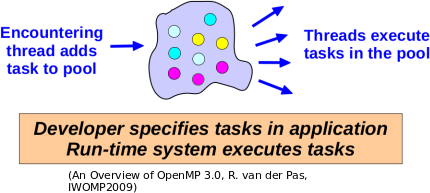
\includegraphics[width=\textwidth]{omp_task_pool.png}
\end{frame}


%%%%%%%%%%%%%%%%%%%%%%%%%%%%%%%%%%%%%%%%%%%%%%%%%%%%%%%%%%% 

\begin{frame}
  \frametitle{Synchronisation des tâches}
  \framesubtitle{Modèle \emph{Fork/Join}}
  

  \begin{block}{Barrières \og normales\fg{}}
    \begin{itemize}
    \item Implicites : à la fin d'une région parallèle, de \texttt{omp for}, ...
    \item Explicites : \texttt{\bf \#pragma omp barrier}
    \end{itemize}

    \medskip
    
    \textbf{Garantie} : Toutes les tâches crées par un thread de l'équipe courante sont
    terminées à la sortie de la barrière
  \end{block}
  
  \bigskip
  
  \begin{exampleblock}{Barrière de tâches : \texttt{\bf \#pragma omp taskwait}}
    \begin{itemize}
    \item La tâche courante attend la terminaison de ses tâches \alert{filles}
    \item Seulement filles directes, pas descendantes
    \end{itemize}
  \end{exampleblock}  
\end{frame}

%%%%%%%%%%%%%%%%%%%%%%%%%%%%%%%%%%%%%%%%%%%%%%%%%%%%%%%%%%%%%%

\begin{frame}[fragile]
  \frametitle{Exemple : parcours d'une liste chainée}

\begin{minted}[fontsize=\small]{C}
struct item_t {
  void * data;
  struct item_t * next;
};
struct item_t * head;
\end{minted}

\begin{columns}[T]
  \begin{column}{0.49\textwidth}
    \begin{block}{Séquentiel}
\begin{minted}[fontsize=\small,stripnl=false]{C}
struct item_t * e = head;


while (e != NULL) {

  process(e->data);
  e = e->next;
}
\end{minted}
    \end{block}
  \end{column}

  \begin{column}{0.49\textwidth}
    \begin{block}{Avec tâches\phantom{Sq}}
\begin{minted}[fontsize=\small]{C}
struct item_t * e = head;
#pragma omp parallel
#pragma omp single
while (e != NULL) {
  #pragma omp task
  process(e->data);
  e = e->next;
}
\end{minted}
    \end{block}
  \end{column}
\end{columns}
\end{frame}

\begin{frame}[fragile]
  \frametitle{Exemple : descente dans un arbre binaire}

\begin{minted}{C}
struct tree_t {
  ...
  struct tree_t *left, *right;
};
struct tree_t *root;
\end{minted}

\begin{columns}[T]
  \begin{column}{0.49\textwidth}
    \begin{block}{Séquentiel}
\begin{minted}[stripnl=false]{C}
void parcours(struct tree_t *t)
{
  ...
  if (t->left) 

      parcours(t->left);
  if (t->right) 

      parcours(t->right);
}


parcours(root);
\end{minted}
    \end{block}
  \end{column}

  \begin{column}{0.49\textwidth}
    \begin{block}{Avec tâches\phantom{Sq}}
\begin{minted}{C}
void parcours(struct tree_t *t)
{
  ...
  if (t->left) 
      #pragma omp task
      parcours(t->left);
  if (t->right) 
      #pragma omp task
      parcours(t->right);
}
#pragma omp parallel
#pragma omp single
parcours(root);
\end{minted}
    \end{block}
  \end{column}
\end{columns}
\end{frame}

%%%%%%%%%%%%%%%%%%%%%%%%%%%%%%%%%%%%%%%%%%%%%%%%%%%%%%%%%%%%%%%

\begin{frame}
  \frametitle{Directive \texttt{omp task}}

  \begin{framed}
  {\tt \#pragma omp task } {\it [clause], [clause], ...}  \\
  {\it bloc structuré} 
\end{framed}

\medskip

Clauses associées :
  \begin{itemize}
  \item  {\tt private} ({\it liste\_de\_variables}), {\tt firstprivate} ({\it
      liste\_de\_variables}), {\tt shared} ({\it liste\_de\_variables})
  \item {\tt default(shared | none)}
  \item {\tt untied}
  \item {\tt depend}({\it dependance-type}: {\it list})
  \item {\tt if({\it expression})}
  \end{itemize}  
\end{frame}

%%%%%%%%%%%%%%%%%%%%%%%%%%%%%%%%%%%%%%%%%%%%%%%%%%%%%%%%

\begin{frame}[fragile]
  \frametitle{Tâches : portée des variables}

  \begin{itemize}
  \item Le plus utile avec les tâches : \textbf{firstprivate}
  \item Attribut \textbf{firstprivate} par défaut sur toutes les variables...
  \item  \alert{\bf sauf} si elles sont déjà considérées comme \textbf{shared}
    \begin{itemize}
    \item Variable globale
    \item Variable déclarée avant la région parallèle
    \item Variable explicitement marquée comme \texttt{shared}
    \end{itemize}
  \end{itemize}

  \begin{alertblock}{\bf Attention aux variables partagées sur la pile}
\begin{minted}{C}
void f()
{
    int i = 3;
    #pragma omp task shared(i)
    printf("%d\n", i);
}

#pragma omp parallel
#pragma omp single
f();
\end{minted}
  \end{alertblock}
\end{frame}

%%%%%%%%%%%%%%%%%%%%%%%%%%%%%%%%%%%%%%%%%%%%%%%%%%%%%%%

\begin{frame}[fragile]
  \frametitle{Tâches : cas où \texttt{shared} est a priori nécessaire}

\begin{minted}{C}
struct tree_t {
  ...
  struct tree_t *left, *right;
};
struct tree_t *root;

/* Renvoie le nombre de noeuds de l'arbre. */
int size(struct tree_t *t)
{
  int s_left = 0, s_right = 0;
  if (t->left)
      #pragma omp task shared(s_left)
      s_left = size(t->left);
  if (t->right) 
      #pragma omp task shared(s_right)
      s_right = size(t->right);
  #pragma omp taskwait
  return 1 + s_left + s_right;
}
#pragma omp parallel
#pragma omp single
printf("%d\n", size(root));
\end{minted}
\end{frame}

%%%%%%%%%%%%%%%%%%%%%%%%%%%%%%%%%%%%%%%%%%%%%%%%%%%%%%%

% \begin{frame}
%   \frametitle{Tâches : ordonnancement}

%   \begin{block}{Liaison tâche $\leftrightarrow$ thread}
%     \begin{itemize}
%     \item Par défaut les tâches sont \textbf{tied} (liées)
%     \item[$\rightarrow$] toujours exécutées par le même thread (celui qui les a crées)
%     \item Tâche suspsendue seulement aux \emph{task scheduling points} :
%       création/terminaison de tâche, barrière, \texttt{taskwait}, \texttt{taskyield}
%     \end{itemize}
%   \end{block}

%   Problème potentiel : déséquilibrage de charge

%   \begin{exampleblock}{Clause \textbf{untied}}
%     \begin{itemize}
%     \item La tâche peut passer d'un thread à l'autre lors d'un \emph{task scheduling point}
%     \item \alert{Attention aux variables \texttt{threadprivate}}
%     \item \alert{Attention à l'indice du thread}
%     \item \alert{Attention aux sections critiques}
%     \end{itemize}
%   \end{exampleblock}  
% \end{frame}

%%%%%%%%%%%%%%%%%%%%%%%%%%%%%%%%%%%%%%%%%%%%%%%%%%%%%%%%%%%

\begin{frame}[fragile]
  \frametitle{Tâches : granularité}

  \textbf{Créer une tâche a un coût non-trivial}

  \bigskip

  \begin{exampleblock}{Ne pas créer des tâches minuscules}
    \begin{itemize}
    \item \emph{Clause} \textbf{if} de la directive \texttt{omp task}
      \begin{itemize}
      \item \texttt{\#pragma omp task if(prof < PROF\_MAX)}
      \item La tâche est \alert{quand même créée}...
      \item ...mais exécutée tout de suite par le thread courant
      \end{itemize}

      \medskip

    \item \emph{Instruction} \texttt{if}:
\begin{minted}{C}
if (prof < PROF_MAX) {
  #pragma omp task
  stuff(...);
} else {
  stuff(...);
}
\end{minted}
      \item[$\rightarrow$] à privilégier a priori
    \end{itemize}
  \end{exampleblock}
  
\end{frame}

%%%%%%%%%%%%%%%%%%%%%%%%%%%%%%%%%%%%%%%%%%%%%%%%%%%%%%%%

\begin{frame}
  \frametitle{Tâches : dépendances}

  TODO...
\end{frame}

%%%%%%%%%%%%%%%%%%%%%%%%%%%%%%%%%%%%%%%%%%%%%%%%%%%%%%%%

\begin{frame}
  \frametitle{Tâches : dépendances}
  \framesubtitle{Exemple de la mort (Christian Terboven)}
  
  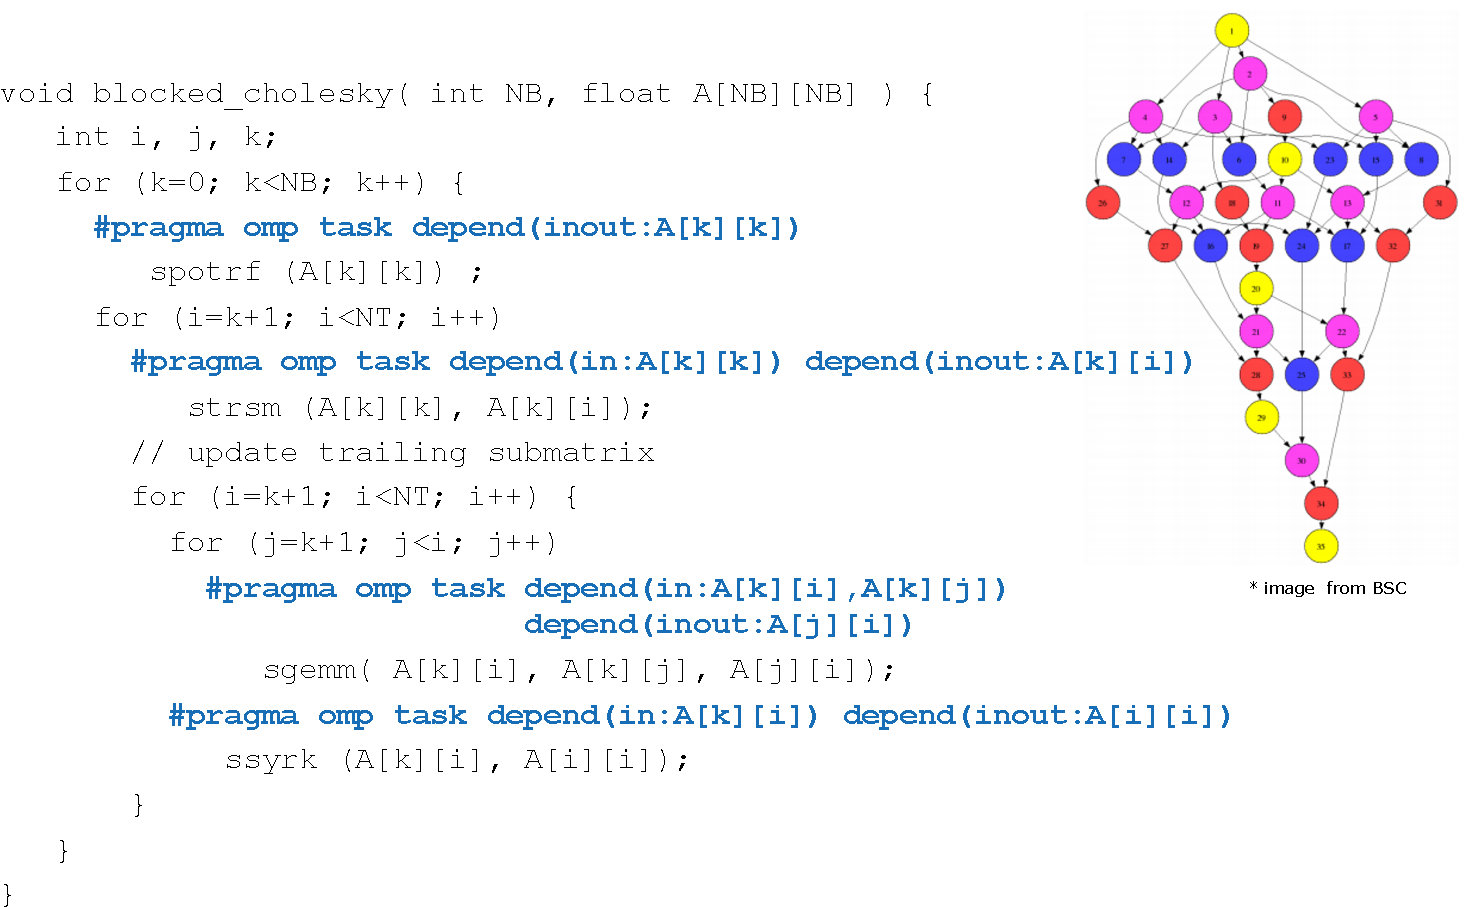
\includegraphics[width=\textwidth]{block_cholesky_tasking}
  
\end{frame}


\end{document}

%%% Local Variables:
%%% TeX-command-extra-options: "-shell-escape"
%%% TeX-engine: xetex
%%% End: